
%(BEGIN_QUESTION)
% Copyright 2006, Tony R. Kuphaldt, released under the Creative Commons Attribution License (v 1.0)
% This means you may do almost anything with this work of mine, so long as you give me proper credit

A device similar to a pneumatic pressure regulator is a pneumatic {\it volume booster} relay:

$$\includegraphics[width=15.5cm]{i00756x01.eps}$$

The purpose of a volume booster is to replicate the same air pressure as the input signal, yet at a greater flow rate than the input signal source would be capable of providing on its own.

Explain how the volume booster works, and why it might be useful in a pneumatic instrumentation system such as this:

$$\includegraphics[width=15.5cm]{i00756x02.eps}$$

\underbar{file i00756}
%(END_QUESTION)





%(BEGIN_ANSWER)

A volume booster installed at the end of a {\it long} pneumatic tube run will significantly improve the valve's response time to any changes in controller output.  Examine the following electrical analogy for a better understanding, where electric charge is the analogue to pneumatic volume:

$$\includegraphics[width=15.5cm]{i00756x03.eps}$$

The tubing's inherent friction to air flow (and the controller's internal restrictions) are analogous to electrical resistance, while the valve actuator's volume is analogous to electrical capacitance.  The two combined form an equivalent RC time constant.

By placing the booster at the end of the tubing run, the controller need not fill or empty such a large volume (the valve actuator) anymore.  The only volume it must control air pressure in now is the volume internal to the booster, which is extremely small.  The booster now handles the pneumatic flow needs of the actuator, and through a much shorter (less restrictive) tubing length.  This greatly decrease the ``RC time constant'' of the system, improving response.

%(END_ANSWER)





%(BEGIN_NOTES)


%INDEX% Basics, pneumatics: pressure booster

%(END_NOTES)


